\documentclass[a4paper, 12 pt]{article}
\author{}
\usepackage{color}
\usepackage[bahasa]{babel}
\usepackage{graphicx}
\title{\textbf{Laporan Tugas Harian Proyek 1}\linebreak}
\date{}
\usepackage{multirow}
\usepackage{enumerate}
\newcounter{saveenumi}
\newcommand{\seti}{\setcounter{saveenumi}{\value{enumi}}} %untuk setting melanjutkan penomoran
\newcommand{\conti}{\setcounter{enumi}{\value{saveenumi}}} %untuk setting melanjutkan penomoran
\usepackage{lipsum}

\begin{document}
	\maketitle
	\begin{center}
		\includegraphics[width=8cm,height=8cm]{logo poltekpos.png}
	\end{center}
	\vspace{0.5 cm}
	
	\begin{center}
		Alwizain Almas Trigreisian \\
		1194004 \\
		D4TI 1A \linebreak
		\newline
		\newline
		\newline
		\linebreak
		\newline
		\newline
		Program Studi D4 Teknik Informatika \\
		Politeknik Pos Indonesia\\
		2019/2020\\
	\end{center}
	
	\newpage
	\begin{flushleft}
		\title{\textbf{Laporan Tugas Harian Proyek 1}}\linebreak
	\end{flushleft}

		\par Pada tanggal 26 Maret 2020, kami barugabung dengan grup bimbingan Mr. Awangga. Setelah itu, kami langsung mendapat tugas dari bapak untuk menginstall navicat dan terkoneksi dengan database mysql. Besoknya sesuai perintah bapak, kami mulai mengerjakan mengisi tabel notfound\_message dan error\_message dengan sistematika setiap kelompok memilih salah satu modul tersebut serta setiap orang harus mengisi 100 record. Bapak member intruksi apabila bingung bisa tanya ke kak inal atau kak wahyu.\\
		
		\par Berikut merupakan cara menghubungkan koneksi ke database mariadb:
		\begin{enumerate}
            \item Membuka \textbf{xampp} dan menjalankan \textbf{MYSQL} serta menyalakan koneksi internet
                \begin{center}
		        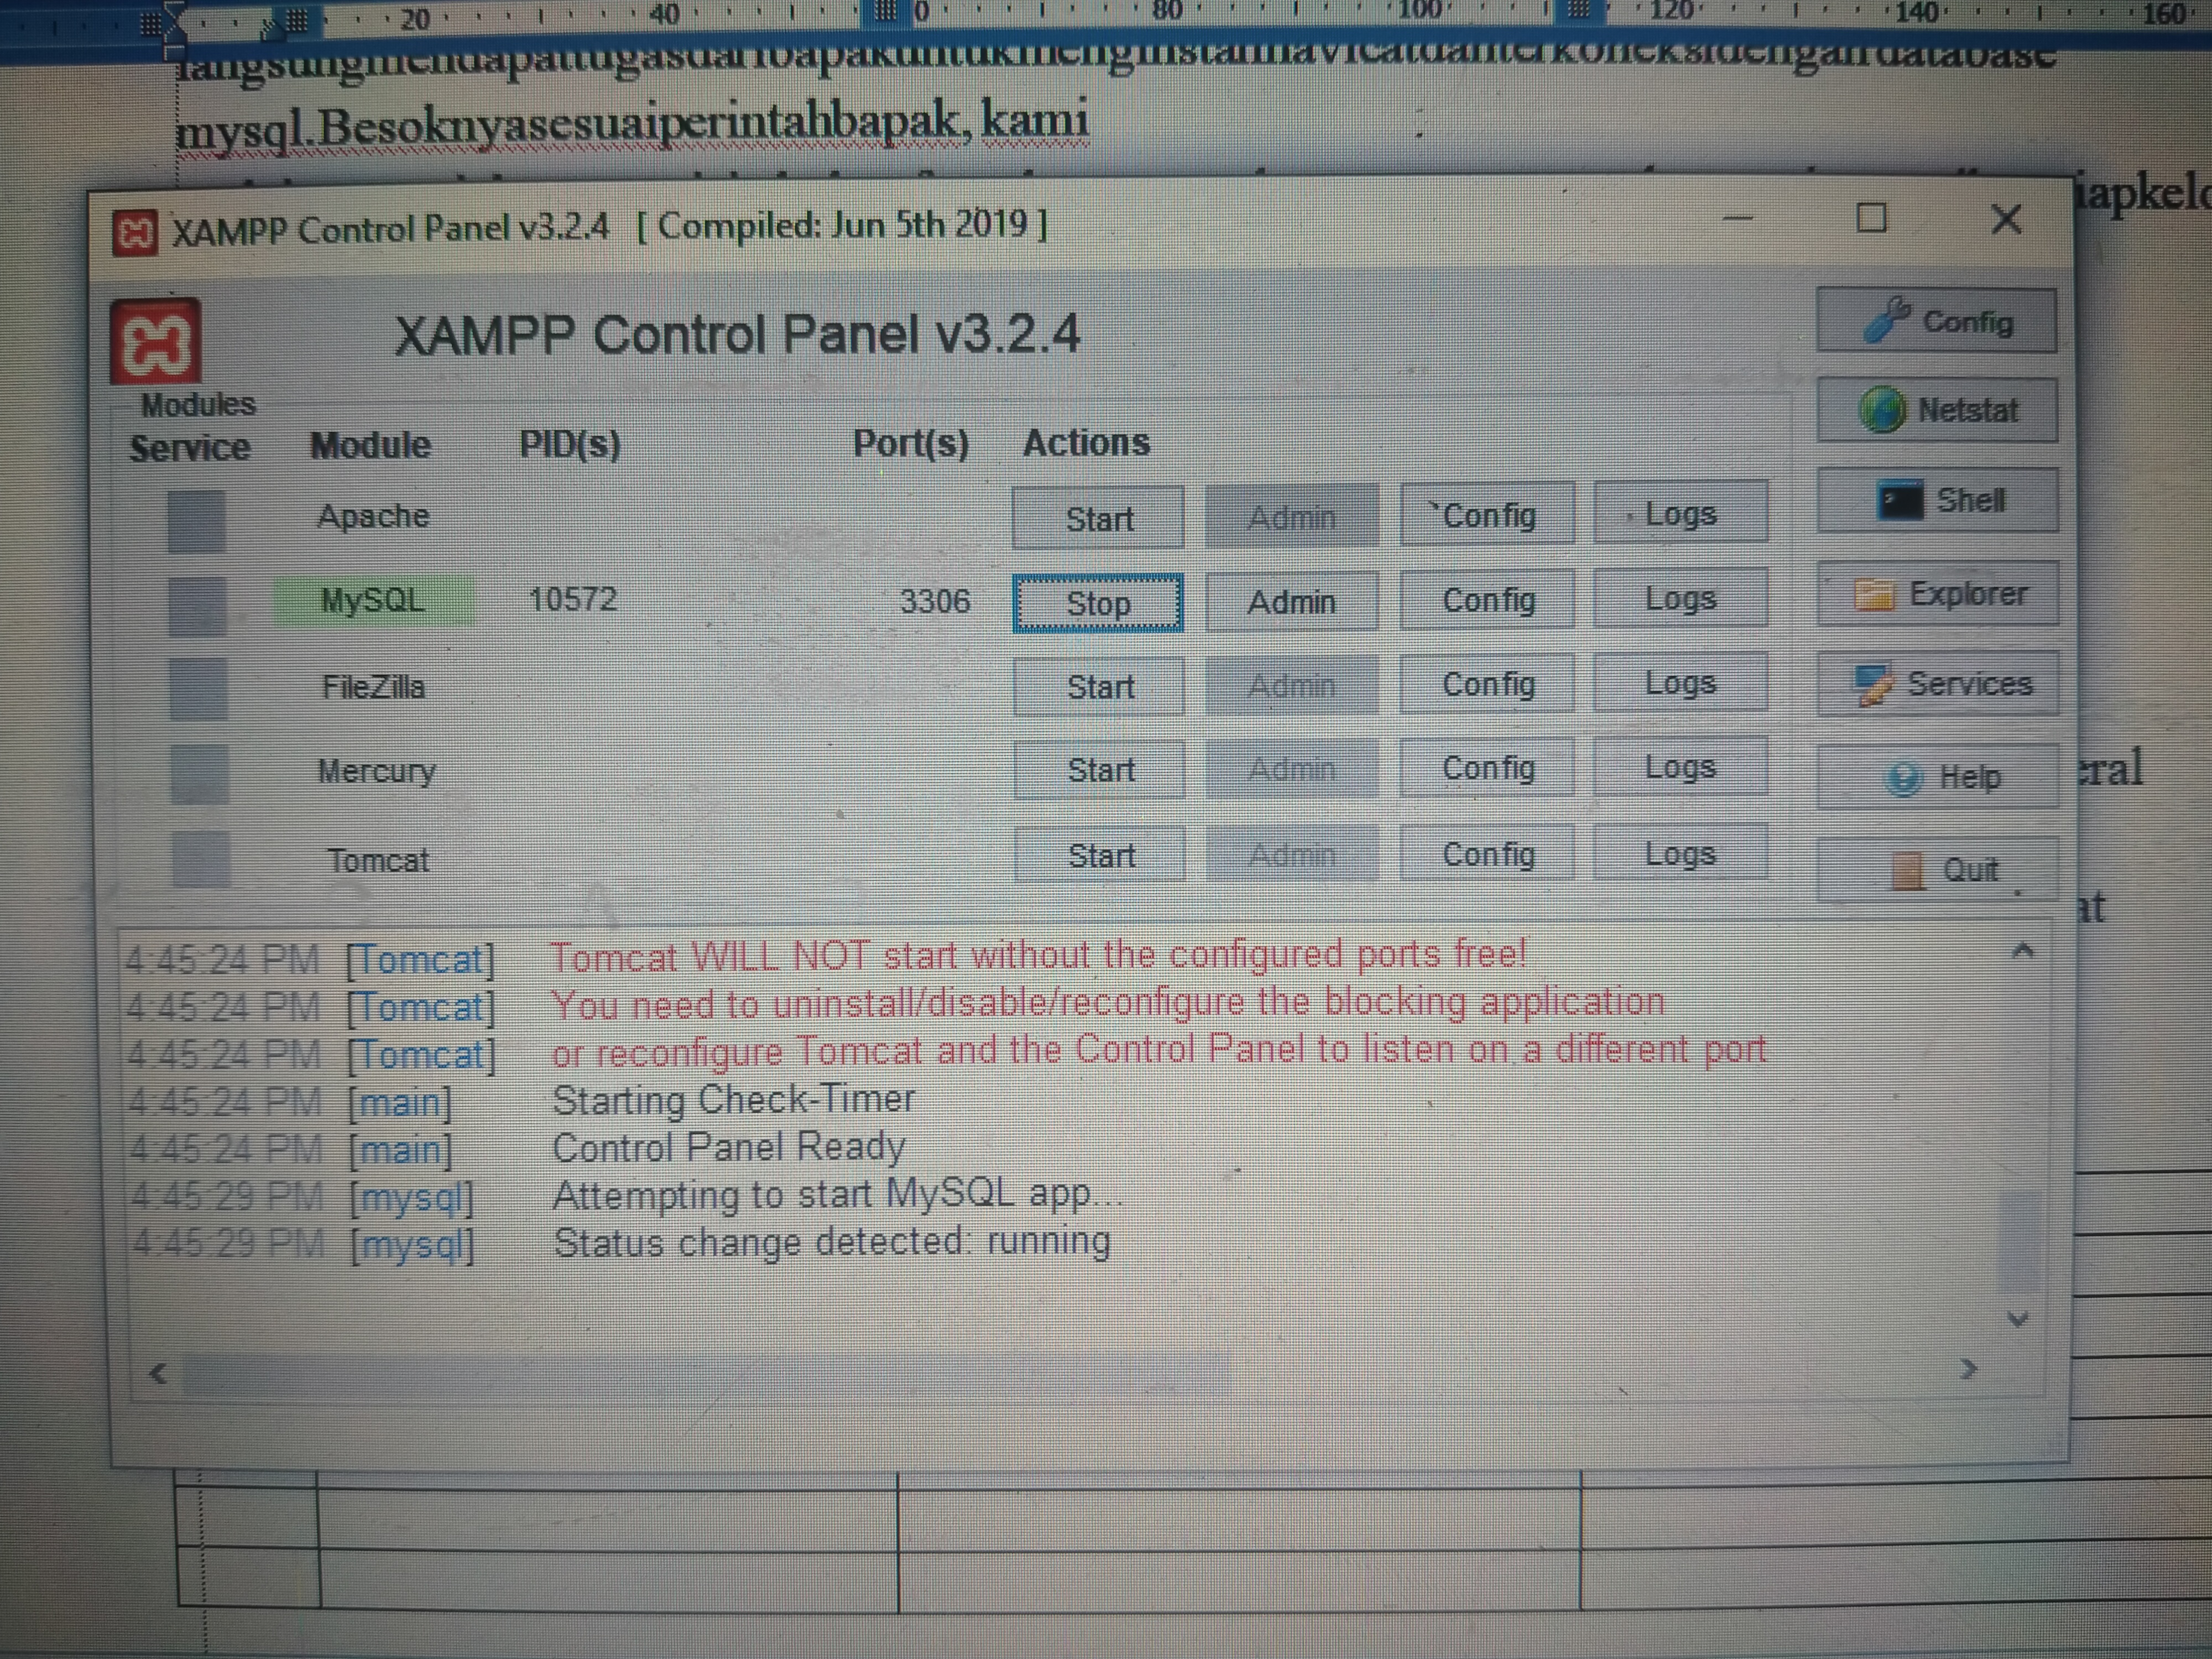
\includegraphics[width=10cm,height=6cm]{IMG20200403012933}
	            \end{center}
            \item Melakukan download dan install Navicat. Setelah itu, membuka \textbf{Navicat} dan pilih \textbf{connection} lalu memilih \textbf{mariadb}
                \begin{center}
		        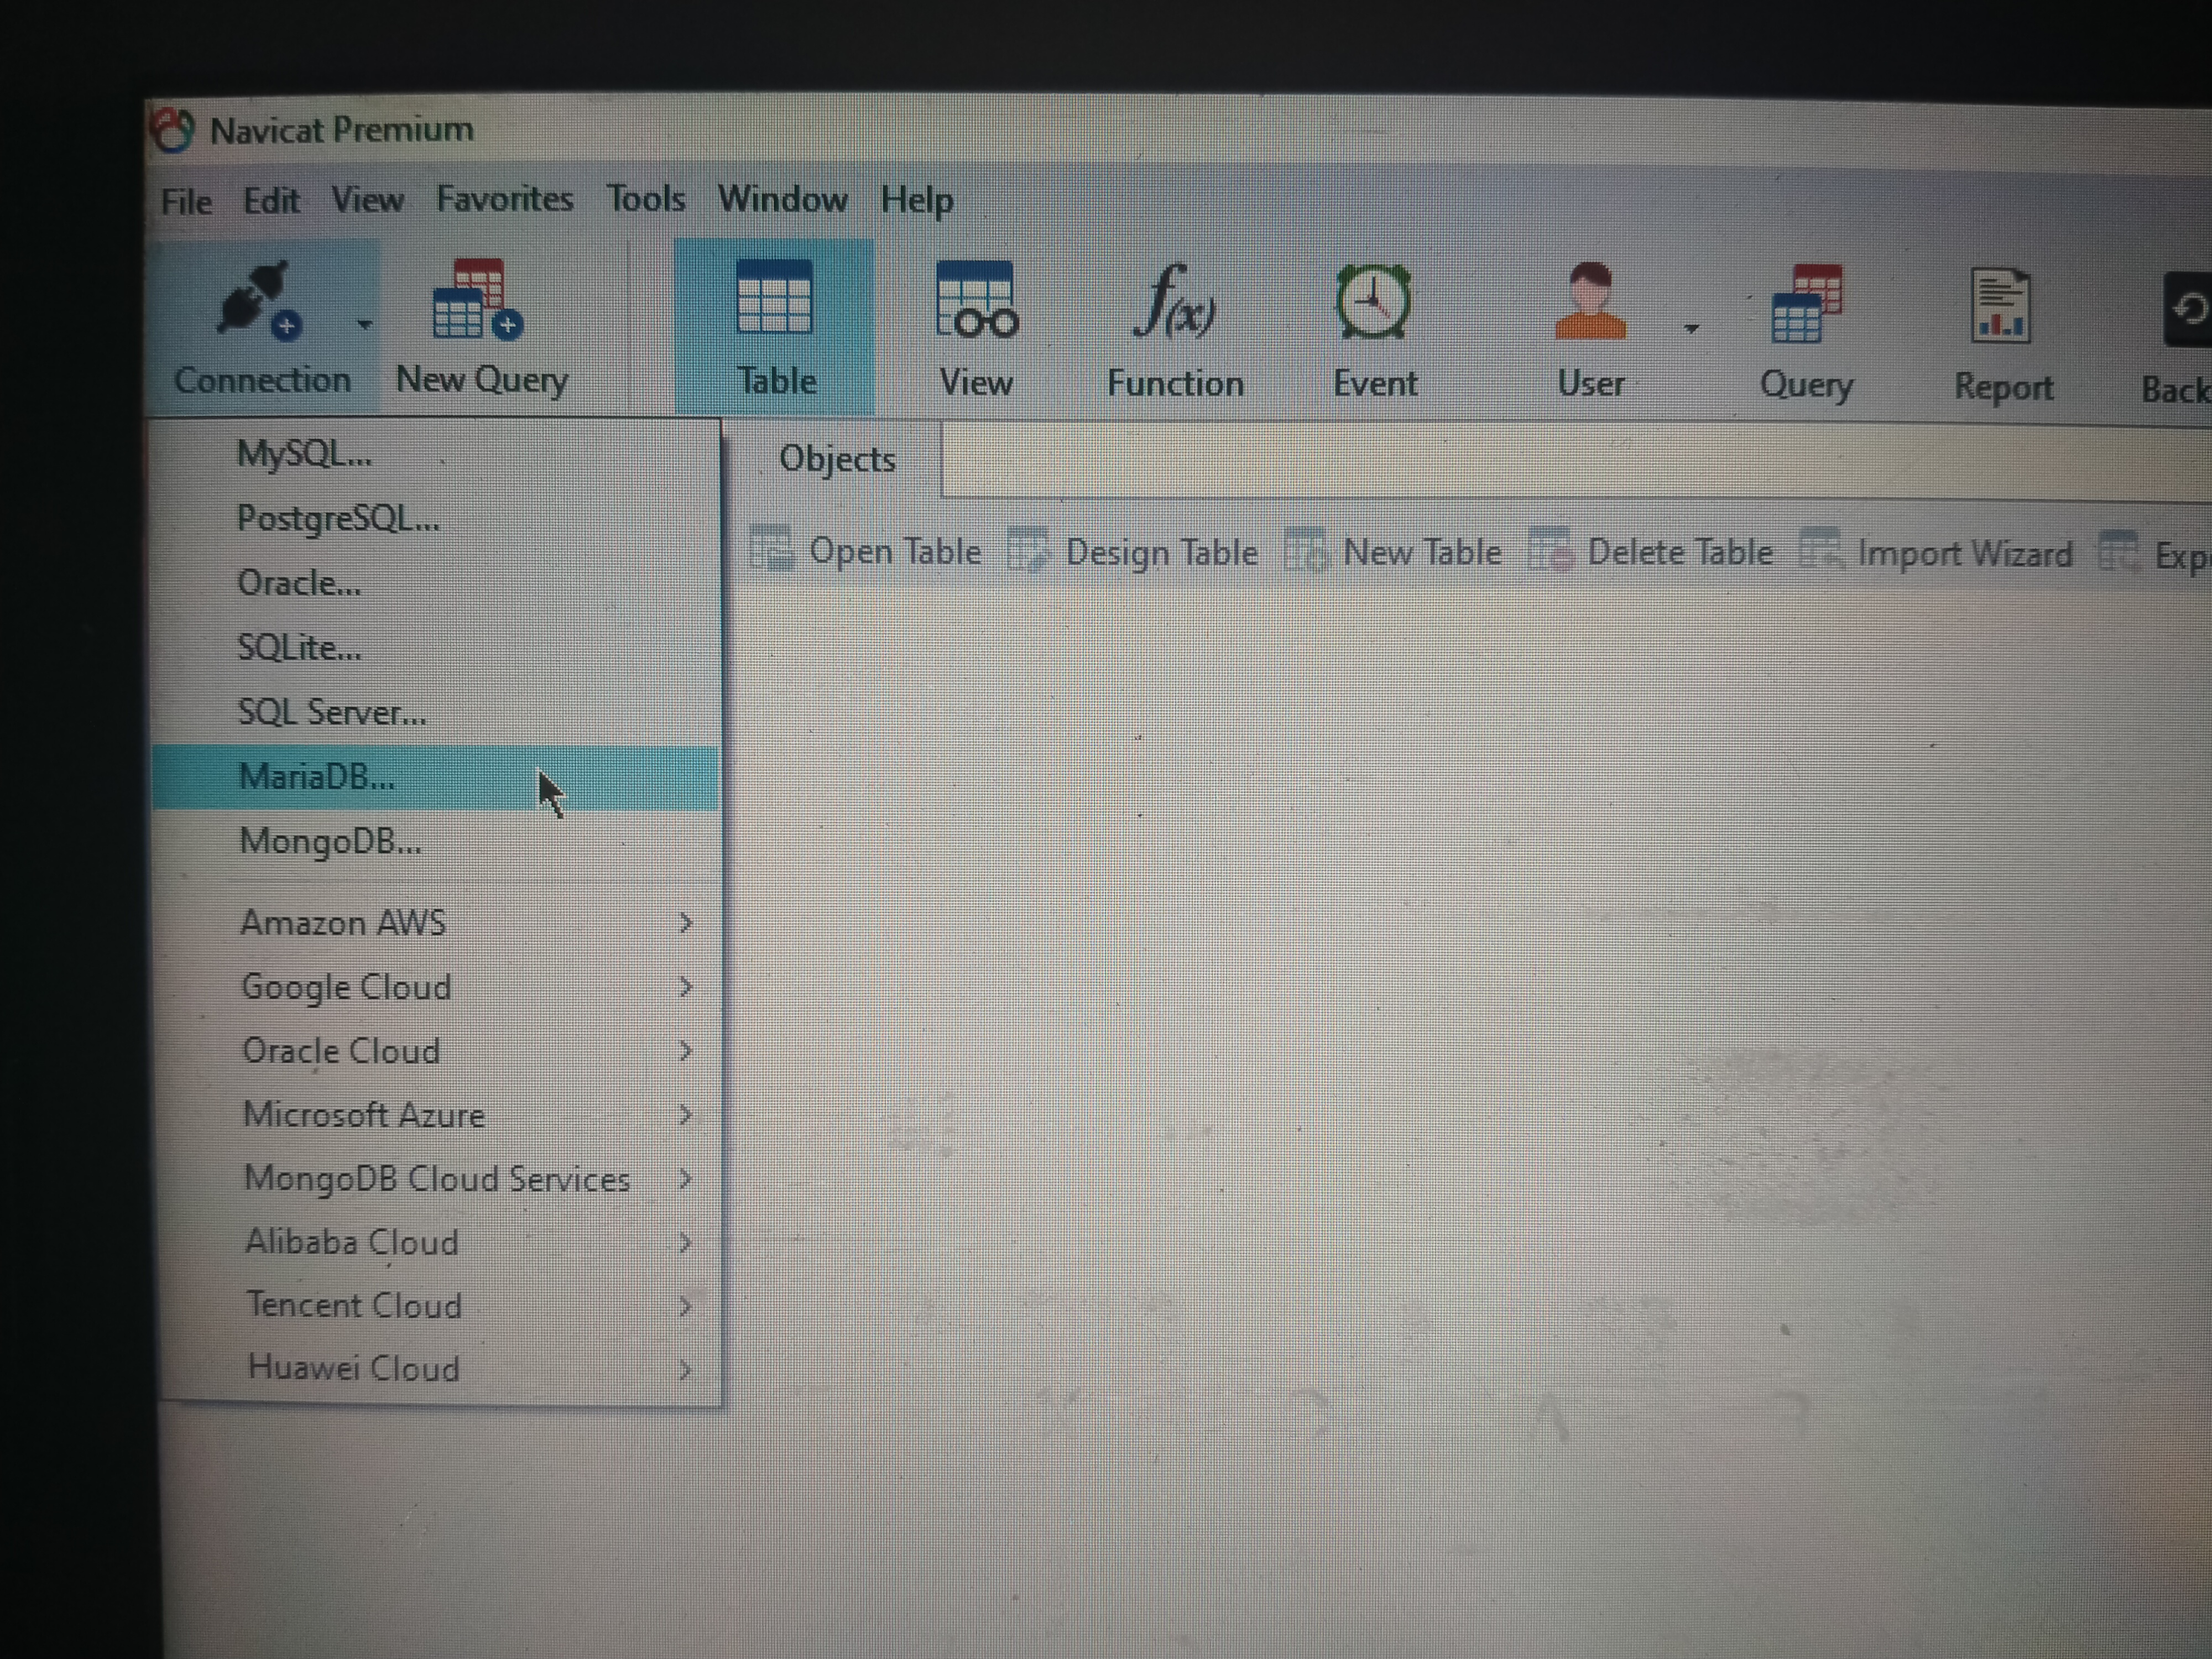
\includegraphics[width=10cm,height=6cm]{IMG20200403013013}
	            \end{center}
            \item Selanjutnya, mengatur koneksi menggunakan \textbf{SSH} terlebih dahulu setelah itu input pada form di \textbf{General}
                \begin{center}
		        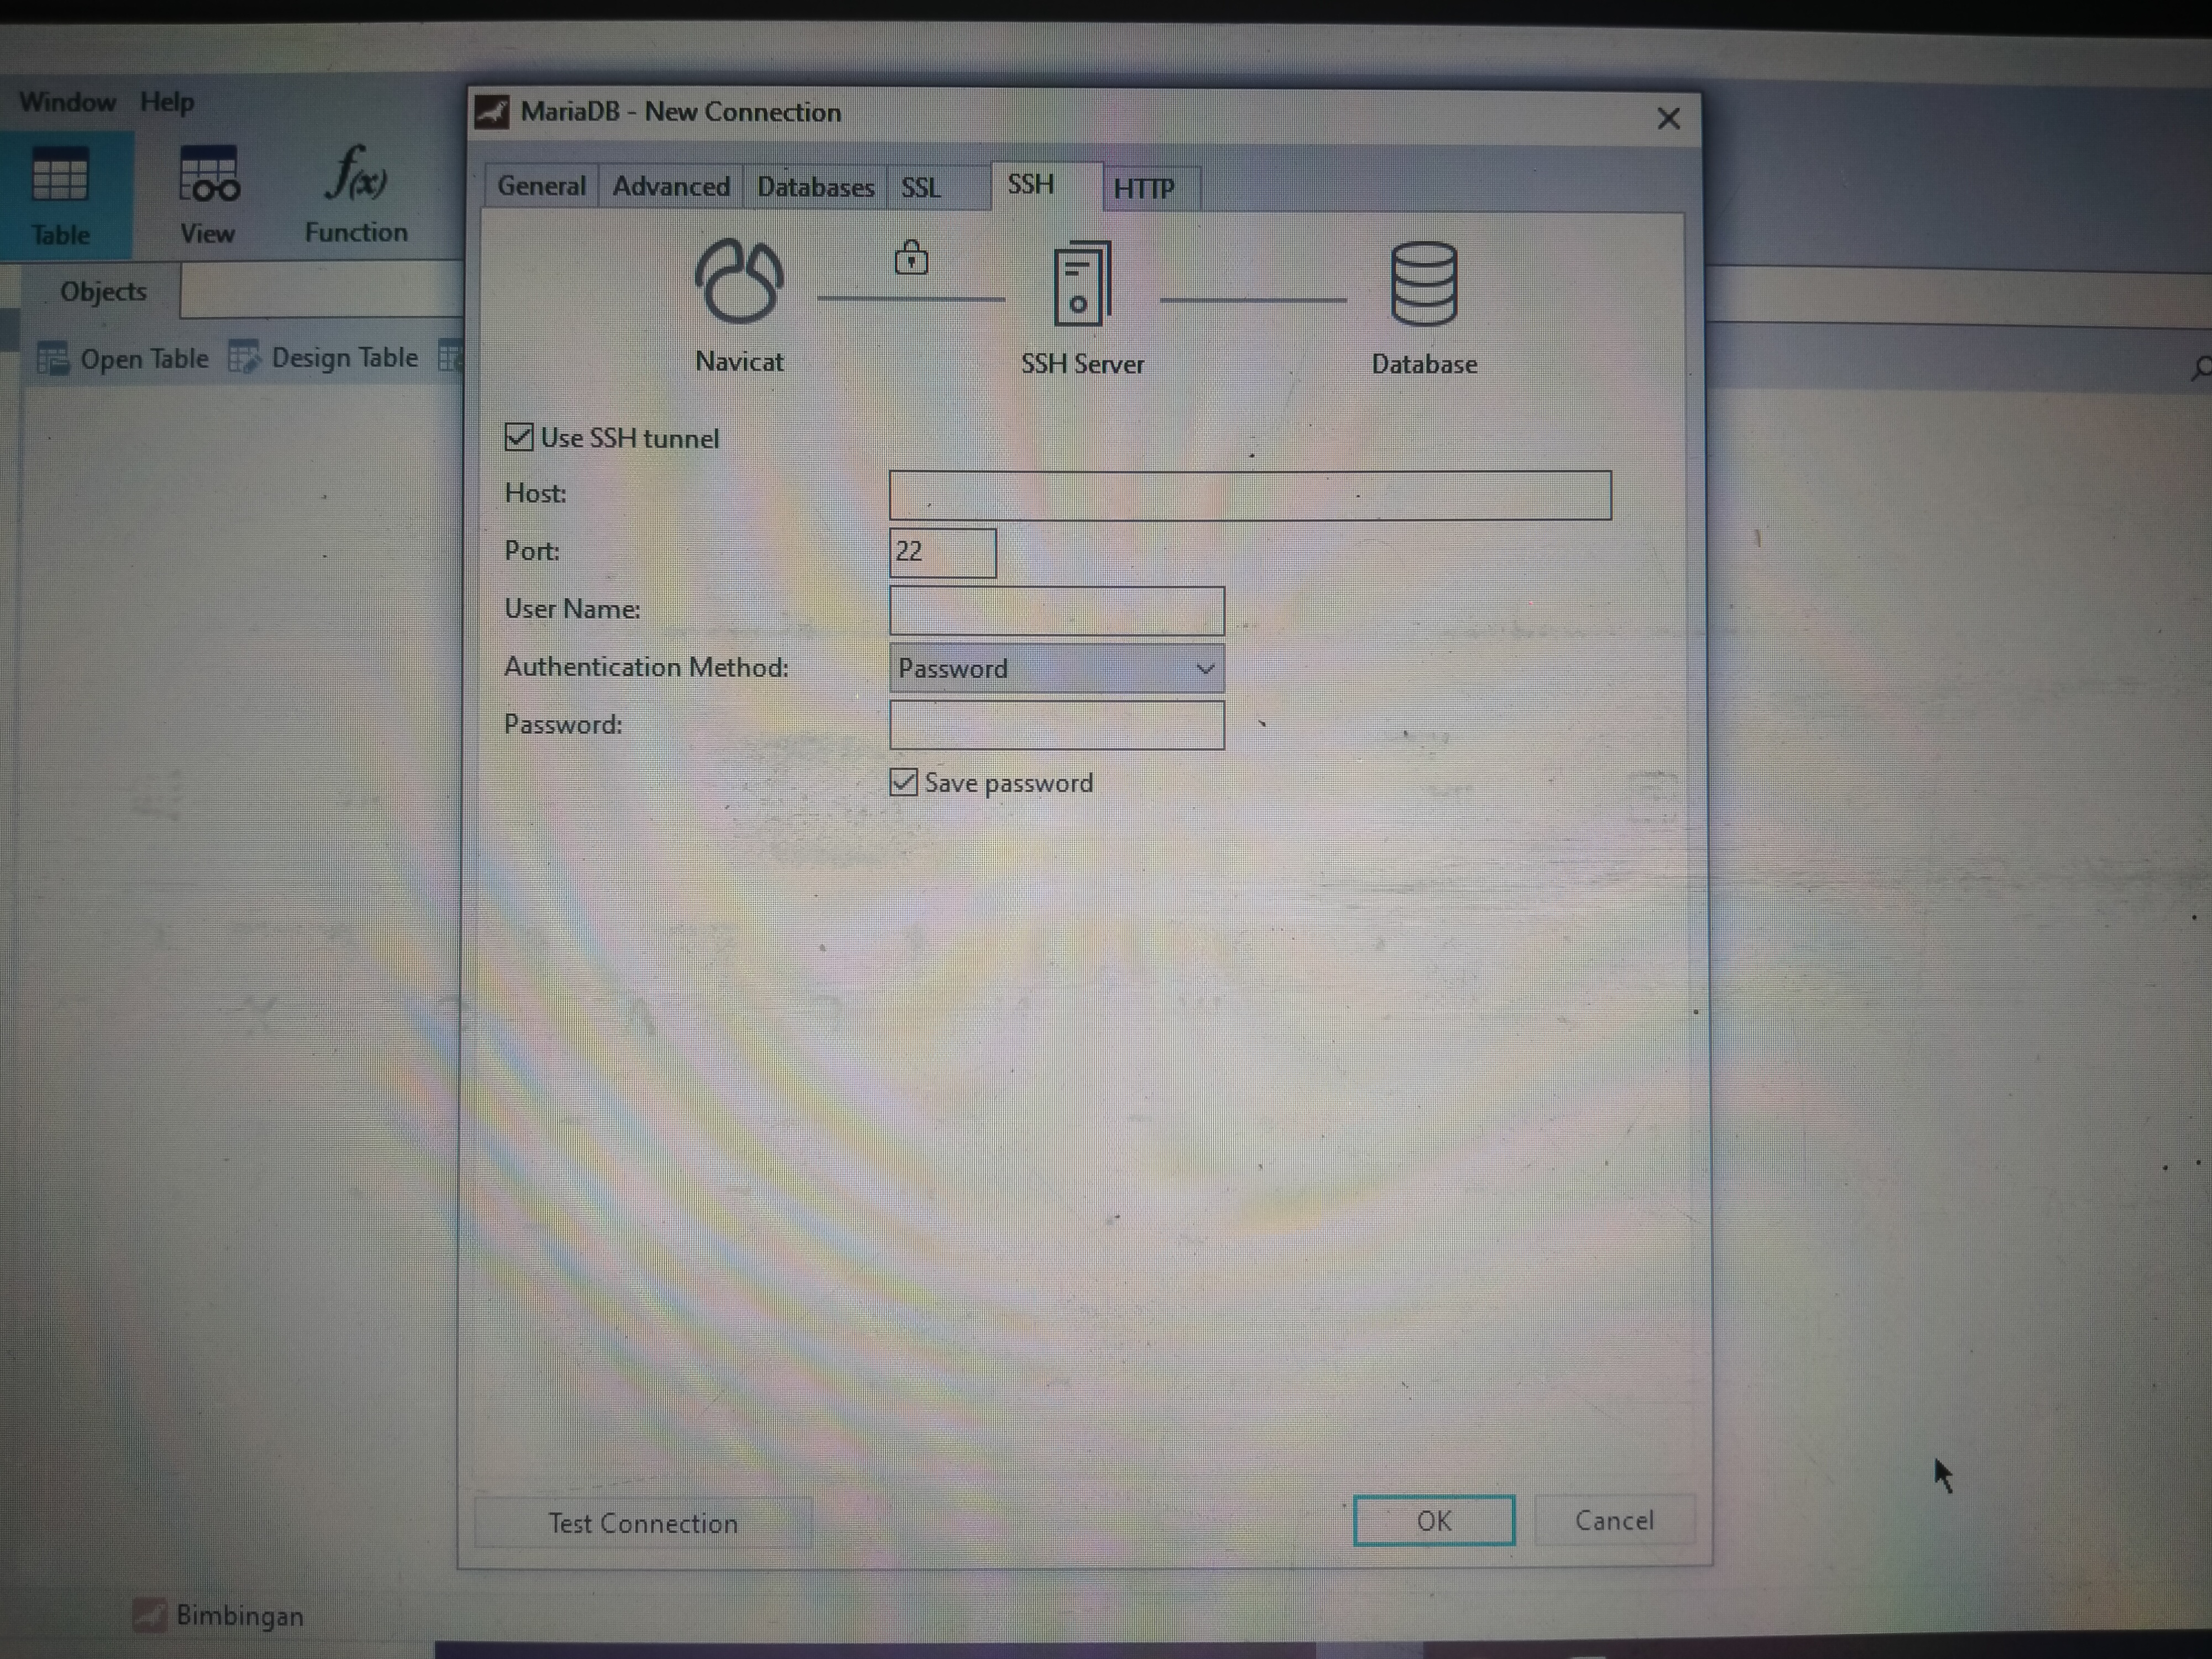
\includegraphics[width=10cm,height=6cm]{IMG20200403013035}
		        \includegraphics[width=10cm,height=6cm]{IMG20200403013048}
	            \end{center}
            \item Setelah koneksi tersambung, maka akan disajikan database yang telah dibuat
                \begin{center}
		        \includegraphics[width=10cm,height=6cm]{IMG20200403013130}
	            \end{center}
            \item Mengisi database tersebut dengan cara memilih tabel yang disediakan dan membuat record baru sesuai dengan gambar berikut,
                \begin{center}
		        \includegraphics[width=10cm,height=6cm]{tutorial}
	            \end{center}
            \seti %harus diketik pada nomor terakhir
        \end{enumerate}

	    \begin{table}[]
            \begin{tabular}{|l|l|l|l|l}
            \hline
                \textbf{No} & \multicolumn{1}{c|}{\textbf{Nama}} & \multicolumn{1}{c|}{\textbf{Penjelasan}} & \multicolumn{1}{c|}{\textbf{Variabel}}  \\ \hline
        
                \textbf{1.} & error\_message & \begin{tabular}[c]{@{}l@{}}error\_message merupakan tabel\\ dalam database bimbingan yang\\ berisikan kumpulan data-data\\ respon dalam menanggapi error\\ dalam aplikasi chatbot Iteung ini.\end{tabular} & \begin{tabular}[c]{@{}l@{}}\#BOTNAME\#\\ Merupakan variabel\\ untuk menyimpan\\ nama chatbot\\ \\ \\ \_\#ERROR\#\_\\ Merupakan variabel\\ untuk menyimpan\\ beberapa error\\ yang terdapat\\ pada aplikasi\end{tabular} \\ \hline
        
                \textbf{2.} & notfound\_message & \begin{tabular}[c]{@{}l@{}}notfound\_message merupakan\\ tabel dalam database\\ bimbingan yang berisikan\\ data-data mengenai respon\\ apabila kata yang\\ dikirimkan oleh pengguna\\ tidak dapat diproses\\ oleh chatbot.\end{tabular} & \begin{tabular}[c]{@{}l@{}}\#BOTNAME\#\\   Merupakan   variabel\\ untuk menyimpan\\ nama chatbot\end{tabular} \\ \hline
        
                \textbf{3.} & opening\_message & \begin{tabular}[c]{@{}l@{}}opening\_message merupakan\\ tabel dalam database\\ bimbingan yang berisikan\\ data-data mengenai respon\\ jawaban apabila pengguna\\ memanggil nama chatbot.\end{tabular} & \begin{tabular}[c]{@{}l@{}}\#BOTNAME\#\\ Merupakan variabel\\ untuk menyimpan\\ nama chatbot\end{tabular} \\ \hline
        
                \textbf{4.} & waiting\_message & \begin{tabular}[c]{@{}l@{}}waiting \_message merupakan\\ tabel dalam database bimbingan\\ yang berisikan data-data respon\\ jawaban yang ditujukan untuk\\ pengguna dengan maksud dan tujuan\\ menyuruh pengguna untuk menunggu.\\ Didalam tabel waiting\_message\\ terdapat beberapa modul,\\ antara lain kelas\_mulai,\\ kelas\_selesai dan jadwal\_kelas\end{tabular} & \begin{tabular}[c]{@{}l@{}}\#BOTNAME\#\\ Merupakan variabel\\ untuk menyimpan\\ nama chatbot\\ \\ \#MATKUL\#\\ Merupakan variabel\\ untuk menyimpan\\ semua matakuliah\\ yang diajarkan\end{tabular}\\ \hline
            \end{tabular}
        \end{table}
        
        \begin{table}[]
            \begin{tabular}{|l|l|l|}
                \hline
                a. kelas\_mulai  & \begin{tabular}[c]{@{}l@{}}kelas\_mulai merupakan module\\ yang terdapat pada\\   tabel waiting\_message juga\\ berupa tabel. Berisi kumpulan\\ data-data respon jawaban\\ yang ditujukan untuk\\ pengguna agar menunggu\\ ketika melakukan perintah\\   “Iteung kelas dimulai”.\end{tabular}   & \begin{tabular}[c]{@{}l@{}}\#BOTNAME\#\\   Merupakan\\   variabel\\ untuk menyimpan\\ nama chatbot\\    \\   \#MATKUL\#\\   Merupakan\\   variabel untuk\\untuk menyimpan semua\\ matakuliah yang diajarkan\end{tabular} \\ \hline
            
                b. kelas\_selesai & \begin{tabular}[c]{@{}l@{}}kelas\_selesai merupakan module\\ yang terdapat pada\\   tabel waiting\_message juga\\ berupa tabel. Berisi kumpulan\\ data-data respon\\   jawaban yang ditujukan\\ untuk pengguna agar\\ menunggu ketika melakukan\\ perintah “Iteung kelas\\ selesai”.\end{tabular} & \begin{tabular}[c]{@{}l@{}}\#BOTNAME\#\\   Merupakan\\   variabel\\ untuk menyimpan\\ nama chatbot\end{tabular} \\ \hline
            
                c. jadwal\_kelas & \begin{tabular}[c]{@{}l@{}}jadwal\_kelas merupakan module\\ yang terdapat pada\\   tabel waiting\_message juga\\ berupa tabel. Berisi\\ kumpulan data-data respon\\   jawaban yang ditujukan\\ untuk pengguna agar\\ menunggu ketika\\ melakukan perintah\\   “Iteung jadwal kelas”.\end{tabular}   & \begin{tabular}[c]{@{}l@{}}\#BOTNAME\#\\ Merupakan variabel\\ untuk menyimpan\\ nama chatbot\end{tabular} \\ \hline
            \end{tabular}
        \end{table}
        
        \newpage
            \par Pada tanggal 28 Maret 2020, kami telah menyelesaikan tugas pertama dari bapak. Setelah itu, bapak langsung menjadwalkan pertemuan via google meet. Dalam meeting tersebut bapak menjelaskan mengenai bagaimana cara menyambungkan navicat ke database mariadb. Setelah itu, bapak juga memberikan contoh bagaimana cara mengisi record. Pada hari itu juga, kami merevisi kerjaan masing-masing karena masih ada kekurangan seperti penggunaan bahasa masih dalam bahasa asing dan ada beberapa evaluasi dari bapak. \linebreak
        
		    \par Pada tanggal 29 Maret 2020, bapak memberikan masukkan untuk memberi emoticon. Setelah itu, kami update record untuk menambahkan emoticon. Selanjutnya, pada tanggal ini bapak merencanakan untuk melakukan pertemuan meeting lagi. Namun, karena ada beberapa hal, meeting pada tanggal ini nggak jadi. \linebreak
		
		    \par Pada tanggal 30 Maret 2020, Bapak merencanakan meeting kembali. Namun, meeting nggak jadi dilakukan karena mungkin ada beberapa hal. \linebreak
		
		    \par Pada tanggal 31 Maret 2020, bapak memberikan tugas kembali untuk melakukan insert pada modul opening\_message. Pada tahap ini, bapak memberi jawaban untuk pertanyaan proyek, yaitu proyek 1 ini setiap orang pegang 1 modul. Setiap orang 1 modul ekisting dan 1 modul pengembangan. Setelah itu, bapak memberi tugas untuk insert record kembali kedalam module\_name, yaitu kelas\_mulai dan kelas\_selesai serta jadwal\_kelas sebanyak 34 record per orang. \linebreak
		
		    \par Pada tanggal 1 April 2020, Bapak menginstruksikan untuk belajar git dan selenium untuk website modul pengembangan dengan kak wahyu dan kak inal. Untuk git harus bisa konfigurasi key SSH antara github dengan desktop. \linebreak
		
		    \par Berikut merupakan cara konfigurasi key git dengan desktop
		        \begin{enumerate}
                    \item Mendownload \textbf{git} melalui link git-scm.com kemudian menjalankan \textbf{git bash} tersebut 
                    \item Sebelumnya, \textbf{buat akun github} terlebih dahulu di www.github.com
                        \begin{center}
                            \includegraphics[width=10cm,height=6cm]{IMG20200403013356}
	                    \end{center}
                    \item Setelah gitbash dijalankan, memastikan dahulu apakah lokasi sudah di home desktop. Apabila belum, cukup ketikkan cd.
                    \item Lalu \textbf{mengetikkan perintah} \\ \textbf{ssh-keygen –t rsa –b 4096 –C “alwizainalmastrigreisian@gmail.com”}
                        \begin{center}
		                    \includegraphics[width=10cm,height=6cm]{IMG20200403013921}
	                    \end{center}
                    \item Selanjutnya \textbf{lihat key} dengan cara \textbf{mengetikkan perintah} \\ \textbf{cat .ssh/id\_rsa.pub}
                        \begin{center}
		                    \includegraphics[width=10cm,height=6cm]{IMG20200403014001}
	                    \end{center}
                    \item Kemudian, \textbf{masuk ke web github} dan pergi ke \textbf{setting}, lalu memilih \textbf{SSH and GPG Keys}, Selanjutnya klik \textbf{New SSH}. Pastekan key dari gitbash ke dalam kolom SSH
                        \begin{center}
		                    \includegraphics[width=10cm,height=6cm]{IMG20200403014038}
		                    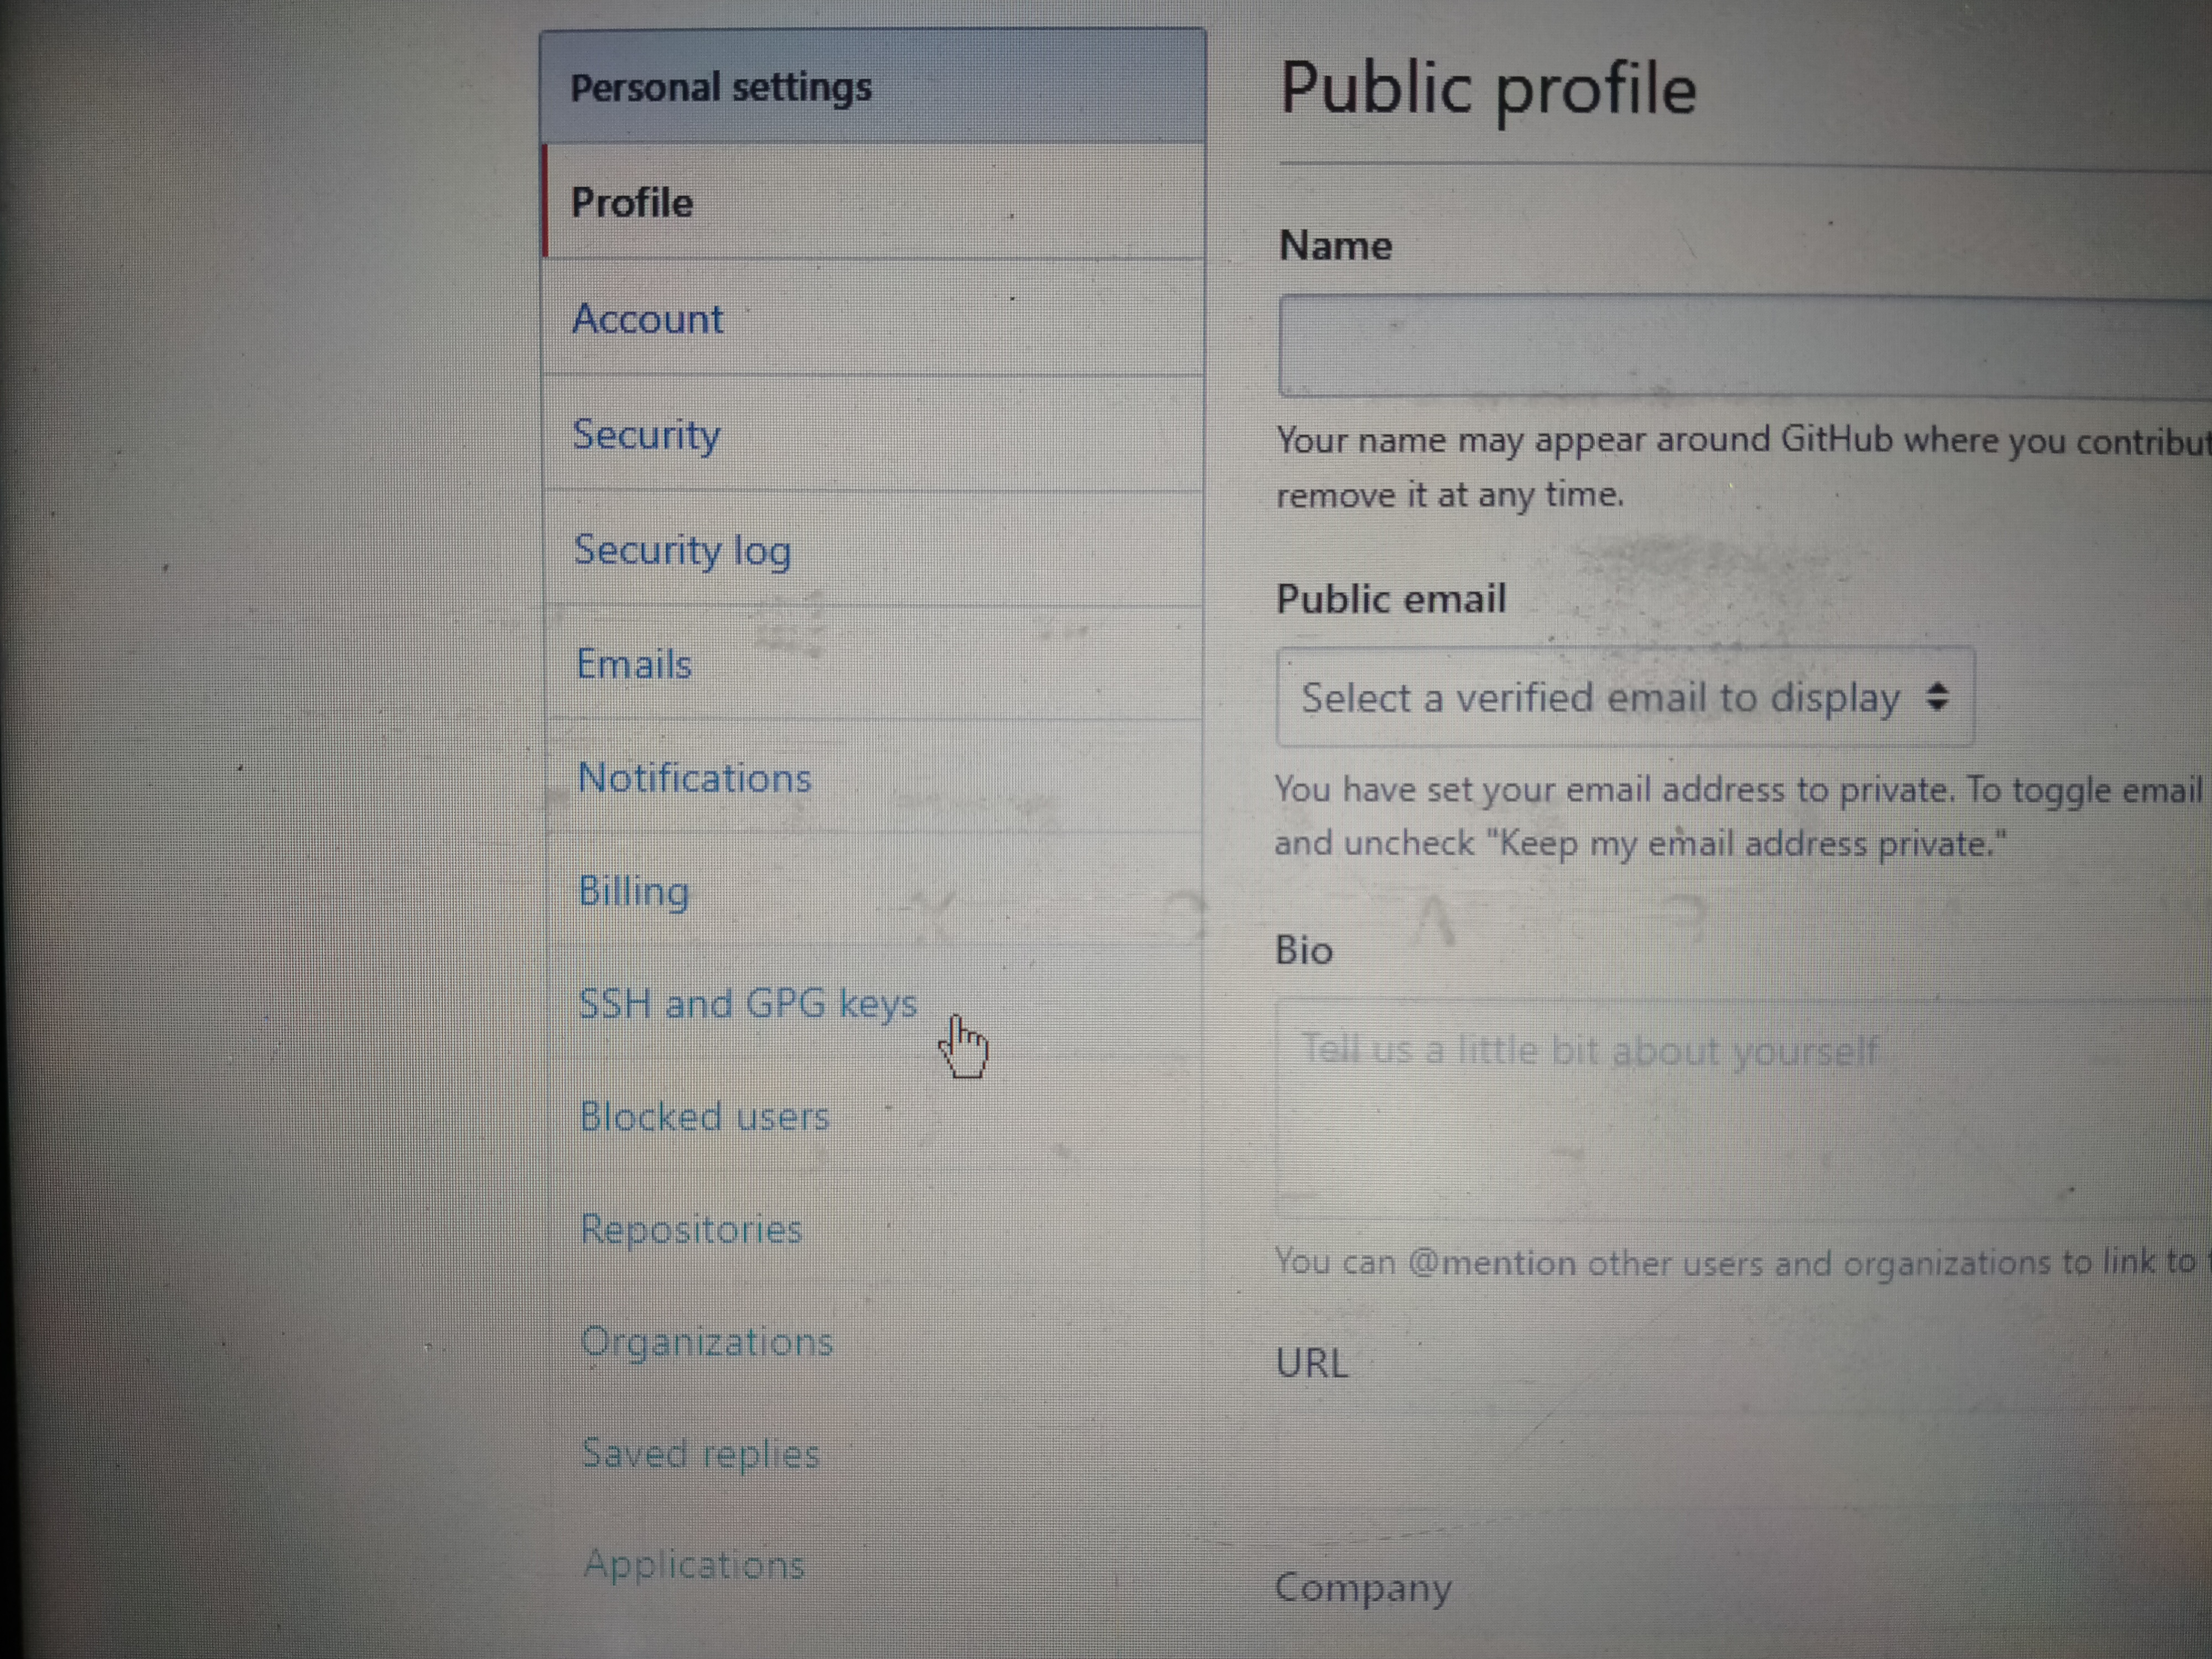
\includegraphics[width=10cm,height=6cm]{IMG20200403014109}
		                    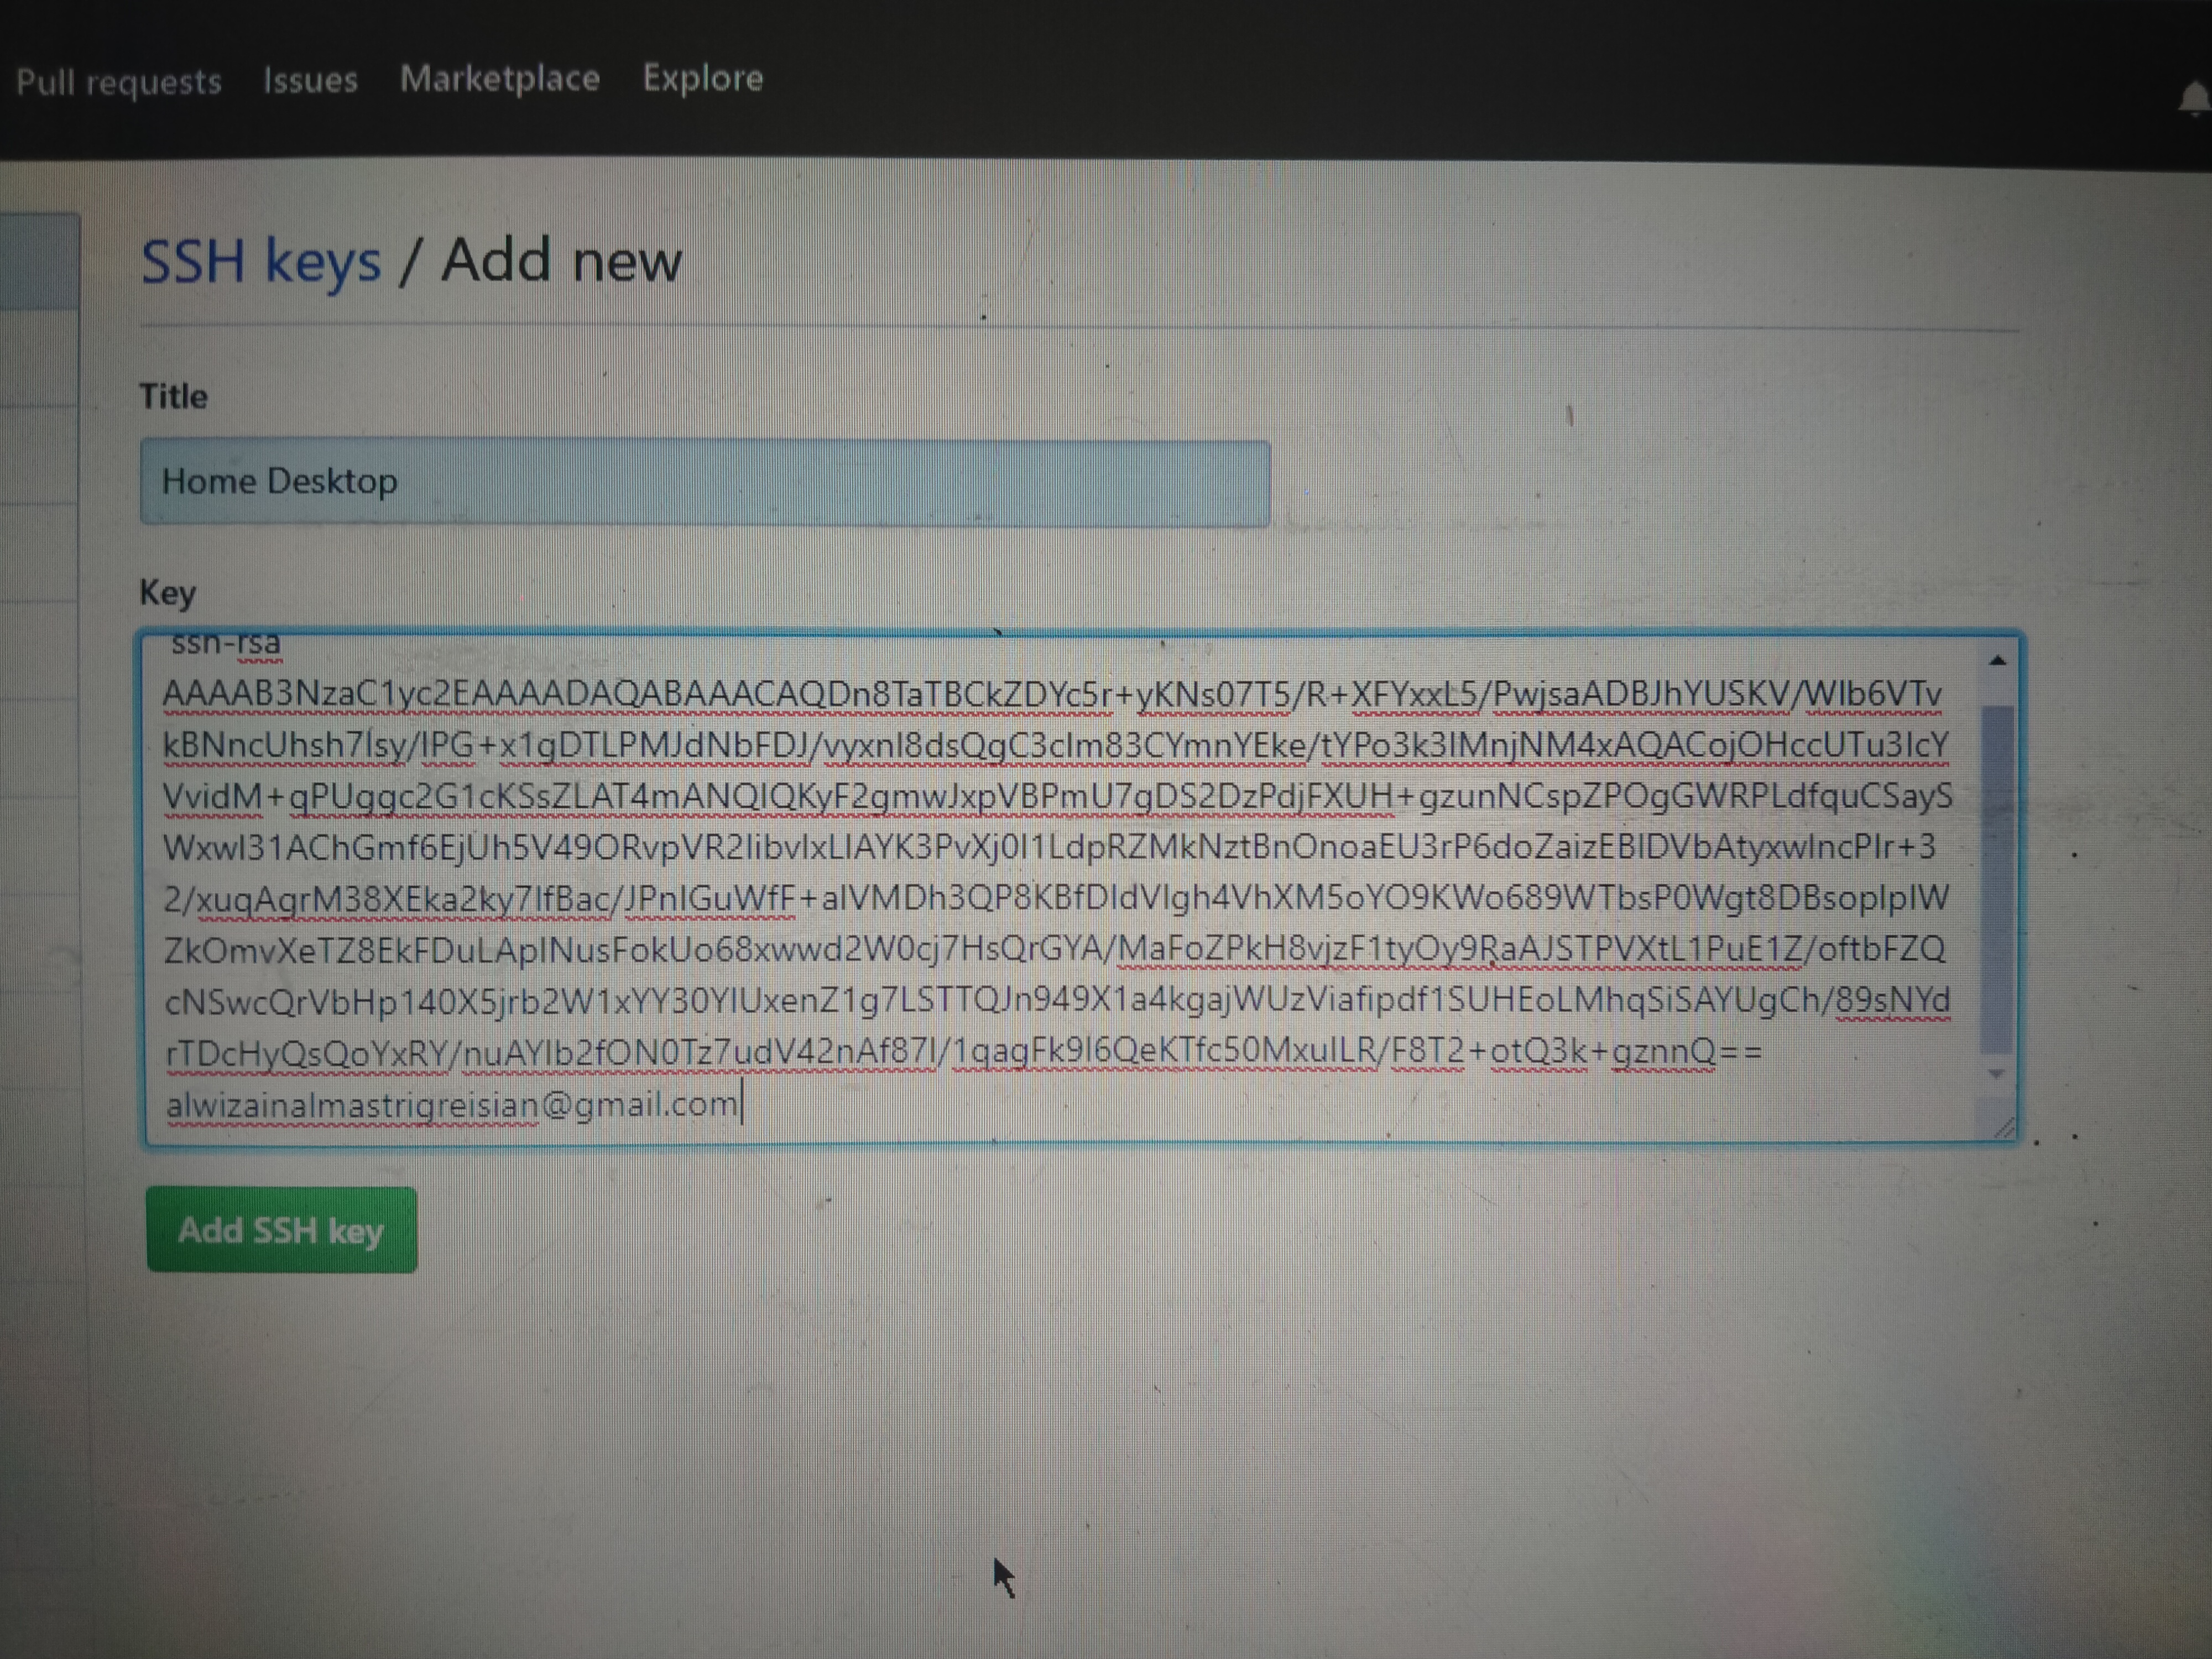
\includegraphics[width=10cm,height=6cm]{IMG20200403014220}
	                    \end{center}
                        \seti %harus diketik pada nomor terakhir
                \end{enumerate}
        
            \begin{table}[h]
            \begin{tabular}{|l|l|l|}
                \hline
                \multicolumn{1}{|c|}{No} & \multicolumn{1}{c|}{Nama} & \multicolumn{1}{c|}{Penjelasan} \\ 
                \hline
                1. & git & \begin{tabular}[c]{@{}l@{}}Git merupakan salah satu\\ alat yang digunakan untuk\\ melakukan pengembangan suatu proyek\end{tabular} \\ 
                \hline
                2. & \begin{tabular}[c]{@{}l@{}}ssh-keygen –t rsa –b 4096 –C\\  “alwizainalmastrigreisian@gmail.com”\end{tabular} & \begin{tabular}[c]{@{}l@{}}Merupakan salah satu\\ perintah untuk menghasilkan suatu\\ kunci atau key SSH dari komputer\\ kita.\end{tabular} \\ 
                \hline
                3. & \textit{cat .ssh/id\_rsa.pub} & \begin{tabular}[c]{@{}l@{}} Perintah ini digunakan untuk\\ menampilkan hasil dari SSH key kita.\end{tabular} \\ \hline
            \end{tabular}
            \end{table}
        
        
            \par Berikut merupakan cara installasi selenium
		        \begin{enumerate}
                    \item Sebelumnya harus \textbf{mendownload dan menginstall anaconda dan chromedriver}. Apabila sudah, maka bisa dilanjutkan installasi ke selenium. 
                    \item Langkah pertama \textbf{installasi anaconda} sampai selesai
                    \item Selanjutnya, \textbf{memindahkan file chrome driver} ke \textbf{C:/windows/System32}
                        \begin{center}
		                    \includegraphics[width=10cm,height=6cm]{IMG20200403014414}
	                    \end{center}
                    \item \textbf{Membuka cmd} dan \textbf{memasukkan perintah} \\ \textbf{pip install selenium}
                        \begin{center}
		                    \includegraphics[width=10cm,height=6cm]{IMG-20200402-WA0051}
	                    \end{center}
                    \item Apabila instalasi selenium sudah selesai, \textbf{membuka Spyder} didalam Anaconda dan \textbf{memasukkan perintah} sebagai berikut, \\ \\
                    \emph{from selenium import webdriver} \\ \emph{from time import sleep} \\ \\ \emph{driver = webdriver.Chrome()} \\ \emph{driver = webdriver.Chrome()} \\ \emph{sleep(2)} \\ \emph{driver.find\_element\_by\_name("username").send\_keys("jhon@gmailcom")} \\ \emph{sleep(2)} \\ \emph{driver.find\_element\_by\_name("password").send\_keys("xxxxxx")} \\ \emph{sleep(2)} \\ \emph{driver.find\_element\_by\_xpath('//*[@id="react-root"]/section/main/article/div[2] /div[1]/div/form/div[4]').click}
                        \begin{center}
		                    \includegraphics[width=10cm,height=6cm]{tutorial2.png}
	                    \end{center}
                    \item Selanjutnya kita \textbf{run} dan otomatis web yang kita tuju akan berjalan.
                        \begin{center}
		                    \includegraphics[width=10cm,height=6cm]{tutorial3.png}
	                    \end{center}
                    \seti %harus diketik pada nomor terakhir
                \end{enumerate}
        
            \begin{table}[h!]
            \begin{tabular}{|l|l|l|}
                \hline
                \multicolumn{1}{|c|}{\textbf{No}} & \multicolumn{1}{c|}{\textbf{Nama}} &  \multicolumn{1}{c|}{\textbf{Penjelasan}}\\
                \hline
                \textbf{1.} & Anaconda & \begin{tabular}[c]{@{}l@{}}Anaconda merupakan platform\\ untuk menggunakan bahasa\\ pemrograman python dan untuk\\ menjalankan selenium. Selain itu,\\ masih banyak lagi\\ aplikasi yang dijalankan\\ dalam Anaconda.\end{tabular} \\ 
                \hline
                \textbf{2.} & Selenium & \begin{tabular}[c]{@{}l@{}}Selenium merupakan sistem otomasi\\ website yang digunakan untuk\\ mencoba menghubungkan antara\\ codingan kita dengan website.\\ Sehingga ketika code\\ dijalankan maka otomatis\\ web akan running sendiri.\end{tabular} \\ \hline
                \textbf{3.} & Chromedriver & \begin{tabular}[c]{@{}l@{}}Merupakan driver untuk menjalankan\\ atau menghubungkan agar\\ otomasi website tersebut\\ terbuka di google chrome.\end{tabular}\\
                \hline
                \textbf{4.} & \textit{pip install selenium} &     \begin{tabular}[c]{@{}l@{}} Merupakan perintah untuk menginstall\\ selenium pada perangkat\\ kita melalui cmd.\end{tabular}\\ 
                \hline
                \textbf{5.} & \textit{from selenium import webdriver} & \begin{tabular}[c]{@{}l@{}}Maksudnya yaitu, kita memerintahkan\\ untuk import webdriver\\ dari selenium agar bisa\\ otomasi web.\end{tabular}\\ \hline
                \textbf{6.} & \textit{from time import sleep} & \begin{tabular}[c]{@{}l@{}}Maksudnya, kita memerintahkan\\ untuk import fungsi sleep\\ dari time dengan tujuan agar\\ nantinya kita dapat\\ memberikan jeda pada\\ saat mengisi form ataupun\\ melakukan fungsi lainnya.\end{tabular}\\ 
                \hline
                \textbf{7.} & \textit{driver = webdriver.Chrome()}
                & \begin{tabular}[c]{@{}l@{}} Memiliki maksud untuk menampung\\ webdriver.Chrome() kedalam\\ variabel driver.\end{tabular}\\ 
                \hline
                \textbf{8.} & \begin{tabular}[c]{@{}l@{}} driver.get("https://www.instagram.com\\ /?hl=id") \end{tabular} & \begin{tabular}[c]{@{}l@{}} Memiliki maksud perintah agar\\ variabel driver mengakses\\ limk yang akan dituju.\end{tabular}\\ 
                \hline
            \end{tabular}
            \end{table}
        
            \begin{table}[h]
            \begin{tabular}{|l|l|l|}
                \hline
                \textbf{9.} & \textit{sleep(2)} &  \begin{tabular}[c]{@{}l@{}}Sleep(2) memiliki arti untuk\\ memberikan jeda selama\\ 2 detik untuk mngisi\\ form atau fungsi lain.\end{tabular}\\
                \hline
                \textbf{10.} & \begin{tabular}[c]{@{}l@{}} driver.find\_element\_by\_name("username").\\ send\_keys("jhon@gmailcom") \end{tabular} & \begin{tabular}[c]{@{}l@{}}Maksudnya yaitu memerintahkan\\ agar variabel driver\\ mencari dan mengisi username\\ dengan menginputkan\\ jhon@gmail.com\end{tabular}\\
                \hline
                \textbf{11.} & \begin{tabular}[c]{@{}l@{}} driver.find\_element\_by\_name("password").\\ send\_keys("xxxxxx") \end{tabular} & \begin{tabular}[c]{@{}l@{}}Maksudnya yaitu memerintahkan\\ agar variabel driver\\ mencari dan mengisi password\\ dengan menginputkan\\ xxxxxx .\end{tabular}\\ 
                \hline
                \textbf{12.} & \begin{tabular}[c]{@{}l@{}} driver.find\_element\_by\_xpath('//*{[}@id=\\ "react-root"{]}/section/main/article/div{[}2{]}\\ /div{[}1{]}/div/form/div{[}4{]}').click \end{tabular} & \begin{tabular}[c]{@{}l@{}}Merupakan perintah untuk\\ mengakses tombol login\\ agar saat kita selesai\\ menginputkan username dan\\ password bisa langsung login\\ ke akun kita\end{tabular}\\
                \hline
            \end{tabular}
            \end{table}
        
            \newpage
            \par Pada tanggal 2 April 2020, Bapak memberi tugas untuk update semua tabel lagi sebanyak 34 per orang dan membuat laporan pekerjaan harian di excel. Hari ini kami juga mendapat target untuk:
		        \begin{enumerate}
                    \item Buka website pake selenium, kode program di push ke repo masing-masing. Setiap orang membuka berbeda website
                    \item Insert kalimat masing-masing tabel 34 row
                    \item Laporan ditaruh digithub. Update di README.md
                    \item Kalo sudah beres kasih tau
                    \seti %harus diketik pada nomor terakhir
                \end{enumerate}
            \par Berikut merupakan penjelasan setiap tugas yang diberikan:
            \begin{enumerate}
                \item Untuk tugas pertama sudah terdapat penjelasan pada tugas tanggal 1 April 2020.
                \item Untuk tugas kedua, saya menginsertkan kalimat atau record kedalam tabel error\_message, notfound\_message, opening\_message, jadwal\_kelas, kelas\_mulai, dan kelas\_selesai. Masing-masing insert tersebut berjumlah 34 row.
                \item Mengupdate README.md dengan laporan insert tabel pada github. Berikut penjelasannya:
                a. Buka repo pada github kemudian tekan tombol fork. Setelah itu copy URL web tersebut. \\
                b. Menentukan folder untuk menyimpan repo dan klik kanan kemudian pilih "Git Bash Here" \\
                c. Mengetikkan perintah git clone https://github.com/InformaticsResearchCenter/Alwizain/sekoteng.git \\
                d. Kemudian folder pada github akan berpindah pada folder yang kita gunakan. Setelah itu, kita dapat mengupdate README.md. \\
                e. Apabila sudah selesai, selanjutnya klik kanan pada layar di folder tersebut. Kemudian masukkan perintah seperti gambar berikut, \\
                f. Refresh halaman website github dan cek apakah file yang kita tambahkan sudah masuk.
                \seti
            \end{enumerate}
            
            \par Pada tanggal 3 April 2020, Bapak Rolly memberikan perintah kepada kami untuk mengupdate jumlah insert tabel yang sudah saya kerjakan pada file README.md di github. Selain itu, bapak juga menjadwalkan meeting melalui Google Meet pukul 1 siang. Namun, mungkin ada beberapa hal yang tidak terduga, meeting tersebut tidak jadi dilaksanakan. \\
            
            \par Pada tanggal 5 April 2020, saya kembali mengupdate laporan jumlah insert tabel pada file README.md dan memberikan alamat website Github Sekoteng kepada Bapak. \\
            
            \par Pada tanggal 6 April 2020, Bapak Rolly memberikan tugas kembali, yaitu:
            \begin{enumerate}
                \item Mengganti kata SIAP menjadi sistem akademik pada seluruh tabel di database.
                \item Insert tabel waiting\_message pada module\_name biodata\_siap\_mahasiswa dan siap\_jadwal dengan masing-masing 20 record per orang.
                \item Insert tabel reply pada keyword panduan dengan masing-masing 10 record per orang.
                \item Pada hari ini, rencana akan melakukan google meet untuk membahas progres proyek 1. Namun, dikarenakan suatu hal, meeting tersebut tidak jadi dilaksanakan.
                \seti
            \end{enumerate}
            
            \par Pada tanggal 7 April 2020, Bapak Rolly memberikan tugas untuk membuka website Telkomsel dan mencoba untuk mengirimkan pesan otomatis kepada Veronika. Selain itu, kita juga diberi tugas untuk input tabel reply berupa pujian, buli, trims, dan joke dengan masing-masing 10 record per orang. \\
            
            \par Pada tanggal 8 April 2020, kami mengupdate laporan insert tabel pada file README.md di Github. Selain itu, kita juga mendapat tugas untuk memperbaiki bahasa Iteung yang masih kasar dan tidak cocok untuk petinggi Poltekpos. \\
            
            \par Pada tanggal 9 April 2020, kami melakukan meeting yang membahas mengenai progres dan cara selenium. Kemudian Bapak juga memberikan tugas kepada kami untuk membuat chatbot pada Telegram serta membuat video tutorialnya yang akan diupload di Youtube dengan deadline hari Senin, 12 April 2020. Selain itu, kami juga mendapat tugas untuk mengganti kata jadwal menjadi absensi pada respon Iteung. \\
            
            \par Pada tanggal 10 April 2020, kami telah menyelesaikan tugas mengganti kata jadwal menjadi absensi pada tabel waiting\_message di siap\_jadwal. \\
            
            \par Pada tanggal 13 April 2020, kami telah menyelesaikan tugas membuat chatbot pada Telegram. \\
            
            \par Pada tanggal 14 April 2020, Bapak Rolly memberikan tugas kepada kita untuk menghubungkan chatbot Telegram yang kita buat dengan Veronika, sehingga kita dapat berkirim pesan dengan Veronika. \\
            
            \par Pada tanggal 18 April 2020, Kak Angga memberikan tugas kepada kita untuk mengisi record masing-masing 20 record pada modul siap\_jadwal dan menambahkan variabel EMAIL. \\
            
            \par Pada tanggal 20 April 2020, Bapak Rolly menyuruh kita untuk melakukan meeting dengan Kak Wahyu dan Kak Inal mengenai penghubungan Veronika dengan Bot di Telegram. \\
            
            \par Pada tanggal 22 April 2020, Bapak Rolly memberikan kami tugas untuk insert record pada tabel waiting\_message dengan modul\_name jadwal\_ujian masing-masing 20 record per orang. \\
            
            \par Pada tanggal 24 April 2020, Bapak Rolly memberikan kami tugas untuk memperbaiki record error\_message yang tertukar ke tabel notfound\_message. \\
            
            \par Pada tanggal 29 April 2020, kami mengajukan bimbingan di web simpro dengan upload file deskripsi aplikasi. \\
            
            \par Pada tanggal 4 Mei 2020, kami mengikuti meeting sidang proyek kakak tingkat. \\
            
            \par Pada tanggal 5 Mei 2020, kami mendapat tugas untuk mengupdate record panduan\_iteung agar dapat menyesuaikan dengan fitur yang terbaru. \\
            
            \par Pada tanggal 6 Mei 2020, terdapat revisi untuk record panduan\_iteung sehingga kami merivisi pekerjaan tersebut. \\
            
            \par Pada tanggal 12 Mei 2020, Saya menanyakan mengenai bagaimana cara Telegram Bot dapat membaca dan mengirim variabel dari sms yang dikirimkan ke nomor hp. Kemudian Bapak Rolly menyuruh kami untuk melakukan google meet dengan Kak Inal, Kak Wahyu, dan Kak Kadek untuk membahas mengenai permasalahan tersebut. \\
            
            \par Pada tanggal 13 Mei 2020, Kami telah menyelesaikan Telegram Bot yang dapat melakukan kirim pesan dengan Veronika. Kemudian Bapak Rolly menyuruh kami untuk membuat vidio demo Telegram Bot tersebut dan diupload di Youtube. Kemudia Bapak Rolly juga menyuruh kami untuk membuat laporan dan sidang. \\
            
            \par Pada tanggal 14 Mei 2020, saya bertanya melalui grup bimbingan mengenai cara pengambilan elemen balasan Veronika karena saya menggunakan xpath biasa tidak bisa. Pada saat itu, saya diberitahu oleh kak Dinda dan kak Angga. Akhirnya saya diberitahu dengan cara copy full xpath dan menambahkan .text dibelakang agar dapat dikonversi menjadi text. Setelah itu, kami mendapat tugas oleh Bapak Rolly untuk membuat video demo part 2 oleh masing-masing individu. \\
            
            \par Pada tanggal 21 Mei 2020, kami laporan kepada Bapak Rolly bahwasannya kami sudah mengirim video demo part 2 ke Youtube. Setelah itu, kami mendapat permintaan untuk membuat dalam mode headless dan perintah langsung dek kuota. Selain itu, kami juga disuruh untuk menambahkan panduan penggunaan Telegram Bot dan mencoba virtual asisten milik maskapai pesawat. \\
            
            \par Pada tanggal 19 Juni 2020, kami disuruh untuk mendaftar pada akun perhutani.com \\
            
            \par Pada tanggal 25 Juni 2020, kami mendapat tugas untuk menyebarkan informasi mengenai webinar Informatic Webinar Series ke adek kelas kami. \\
            
            \par Pada tanggal 26 Juni, saya mendapat tugas untuk mendesain sertifikat dari kegiatan webinar tersebut. \\
            
            \par Pada tanggal 2 Juli 2020, saya berdiskusi dengan Bapak Rolly mengenai penyusunan laporan Proyek 1. Pada akhirnya, Bapak menyuruh saya untuk meminta laporan proyek 2 dari kak Dinda. Pada hari itu juga saya meminta laporan proyek kepada kak Dinda. \\
            
            \par Pada tanggal 3 Juli 2020, kami mengikuti kegiatan webinar yang sudah direncanakan tersebut. \\
            
            \par Pada tanggal 9 Juli 2020, kami mengupload beberapa bab laporan proyek 1 kami di website Simpro. \\
            
            \par Pada tanggal 15 Juli 2020, kami mengupload sisa laporan proyek 1 kami yang sudah selesai. Dengan begitu, laporan proyek 1 kami yang harus diupload di web simpro pada hari ini sudah terselesaikan. \\
            
            \par Pada tanggal 16 Juli 2020, kami mengupload tutorial pembuatan telegram bot veronika ke github dan kami laporkan ke Bapak Rolly juga. \\
            
            
\end{document}
    
    